% define document type, font-size, and paper dimensions
\documentclass[11pt, letterpaper]{article}
% set up image package & path
\usepackage{graphicx}
% subcaption for multi-figures
\usepackage{subcaption}
% adds a header onto every page
\usepackage{fancyhdr}
% adds indent to paragraph after section header
\usepackage{indentfirst}
% make margins 1in
\usepackage[total={6.5in,8.75in},
top=1.25in, left=1in]{geometry}
% add hyperlinks
\usepackage{hyperref}
% adjusting figures
\usepackage{float}

\makeatletter
\setlength{\@dblfptop}{0pt}
\setlength{\@dblfpbot}{0pt plus 1fil}
\makeatother

% set up page style & graphic path
\pagestyle{fancy}
\graphicspath{{./images/}}

% Resize table rows
\renewcommand{\arraystretch}{1.75}

% Set up title page
\renewcommand{\maketitle}{
    \begin{titlepage}
        % Set up title page
        \centering
        \huge{\textbf{The Effects of Sleep on Stress}} \par
        \vspace{.5cm}
        \large{\textbf{ECS 171 Machine Learning}} \par
        \vspace{.5cm}
        \large{\textbf{Group 10 Project Report}} \par
        \vspace{.5cm}
        % group leader
        \large{Leader: Ryan Yu} \par
        \vspace{.5cm}
        % group members
        \normalfont{Amira Basyouni, Calvin Chen, Alexis Lydon, Tianming Tan} \par
        \vspace{.5cm}
        % github repo
        \normalfont{Github Repository: \url{https://github.com/ryyu444/ECS-171-Group-Project} \par}
        \vspace{.5cm}
        % date
        \today
    \end{titlepage}
}

\setlength{\emergencystretch}{3em}

% set up header
\fancyhf{} % clear all header and footer fields
\lhead{The Effects of Sleep} % left header
\rhead{\thepage} % right header
%\fancyhfoffset[LR]{1cm} % increase left, right margin by 1cm

\begin{document}
    \maketitle
    
    \newpage

    \twocolumn
    \section*{Introduction and Background}
    \noindent As a student, we constantly grapple with numerous stressors while striving for academic success. Deadlines, exams, and the intrinsic self-asserted pressure to excel, they all contribute to the challenges we face. These factors can have a negative impact on our quality of learning and thus hinder our progress toward acquiring a degree to ultimately enter the workforce. In contrast, sleep is an activity that we all partake in and seems relaxing. So we posed a question: does sleep have any connections to stress? And if so, how are they related? Our goal is to construct predictions regarding the effects that sleep quality and sleep duration can have on our stress levels. By analyzing our data, we will be able to determine the correlation between stress and those two sleep-related attributes. It’s worth noting that our data includes individuals of ages 27 to 59. Although the range does not fall within the typical college student age, our results can still provide valuable insights and promote awareness that can benefit us for years to come. \\

    \noindent In this machine learning project centered on the intersection of sleep health and stress, our primary objective is to examine the correlation between key attributes such as sleep duration and sleep quality, and their influence on stress levels. This analysis will help us better understand and predict the dynamics between stress and other factors. Thus, it will help identify the attributes that have the most significant impact on stress levels. As an integral part of the project, we will develop accurate models for stress prediction based on the highly correlated attributes in our dataset.
    
    \section*{Literature Review}
    \noindent Machine Learning has great capabilities within the realm of pattern recognition and categorization; two fields that we hope to utilize as we explore the connection between sleep and stress. It is important to address some of the pre-existing studies which were conducted with a similar objective. Presented below are examples of such research and methodologies as well as their overall findings.\\
    
    \noindent Jayawickrama and Rupasingha, researchers from Sabaragamuwa University of Sri Lanka, conducted a study to examine the impact of sleep habits on stress levels.\cite{bib:2} They applied various machine learning models which included Naïve Bayes, Random Forest, Decision Trees, Multi-layer Perceptrons (MLPs), Support Vector Machines (SVMs), and Logistic Regression mixed with cross-validation. It was revealed that five of the six models achieved accuracy rates exceeding 80\%, suggesting that there is a strong correlation between sleep and stress. Notably, Naïve Bayes was the best predictor with an accuracy of 91.27\%.\\ 
    
    \noindent Minhazur Rahman and a different group of researchers predicted stress levels using data collected from sleeping participants.\cite{bib:1} Some of the models they utilized include Gradient Boosting, Decision Trees, Random Forest, Gaussian Naive Bayes, and Linear Support Vector Machine. Their models achieved an accuracy rate of over 95\%, with Naive Bayes and SVM as the top performers.\\
    
    \noindent Overall, these studies highlight the efficacy of machine learning models in predicting stress levels based on sleep data, with Naive Bayes and SVM demonstrating high performance. We hope to utilize these research metrics as the basis of judgment for the models that we will be building and testing.


    \section*{Dataset Description and Exploratory Data Analysis}
    \noindent The dataset being used in this project is titled “Sleep Health and Lifestyle Dataset”\cite{bib:3} and was made by Laksika Tharmalingam, accessible on Kaggle. The dataset comes in the form of a CSV file and contains 400 rows and 13 columns, consisting of various sleep and lifestyle variables (e.g. gender, age, occupation, sleep duration, sleep quality, and stress levels). These variables encompass the very aspects of sleep and health that can be useful in predicting stress. Despite the abundant source of data, a limitation of this dataset is its synthetic nature, generated artificially rather than from real-world observations. Although it may lack certain real-world nuances, high-quality synthetic data proves effective in emulating real datasets. It serves as a cost-efficient and time-saving approach in comparison to gathering real-world observations to use for training and testing machine learning models.\\
    
    \noindent Initially, we conducted essential data preprocessing to convert all categorical data into numerical values, enhancing their compatibility with prediction models. This involved applying label encoding to categorical attributes from the dataset like BMI and Gender. We opted for label encoding over one-hot encoding to both maintain consistency in the number of columns in our dataset and to enhance clarity in visualizing a pair plot and correlation matrix.\\
    
    \noindent Following data preprocessing, we generated a pair plot matrix (\hyperref[fig:pairplot]{Figure~\ref*{fig:pairplot}}) to investigate any potential linearly separable relationships between the attributes and Stress Level. The pair plot revealed notable linear associations, particularly between Sleep Quality and both Sleep Duration and Age in predicting Stress Level. Additionally, Sleep Duration and Gender also have somewhat of a linear relationship in predicting stress.\\
    
    \begin{figure}[H]
        \centering
        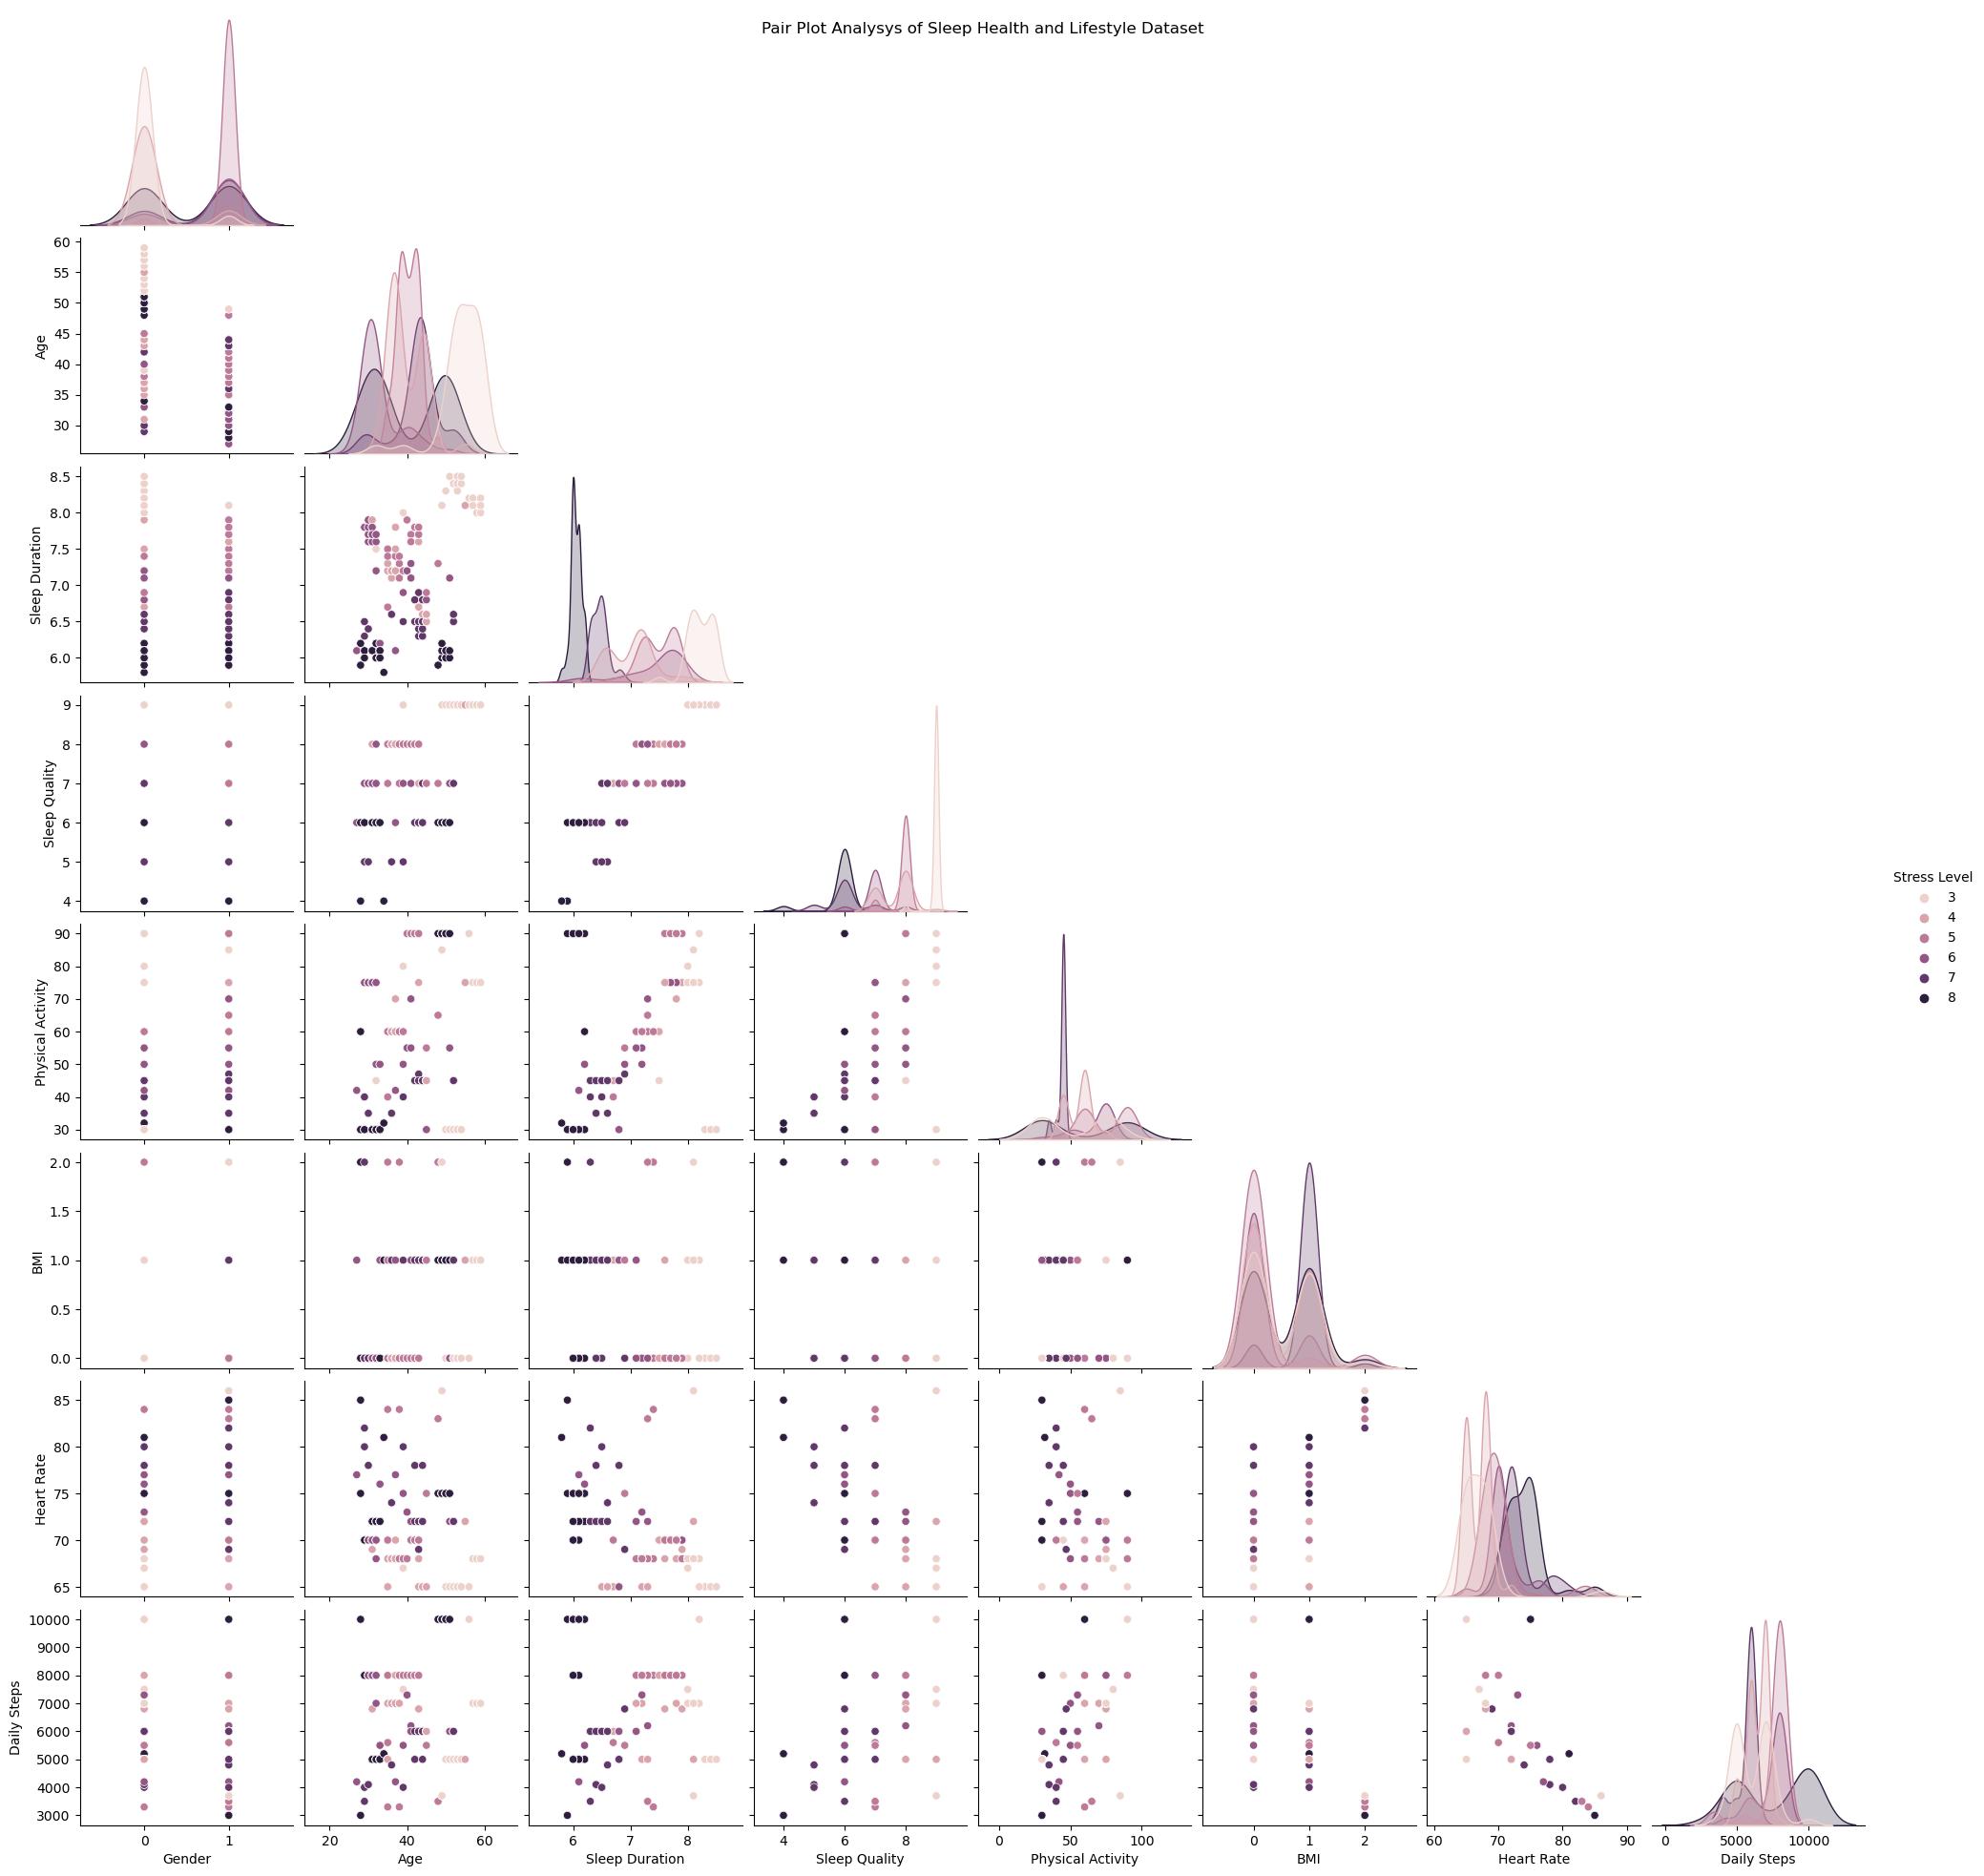
\includegraphics[width=0.40\textwidth]{pairplot.png}
        \caption{Pair Plot Matrix}
        \label{fig:pairplot}
    \end{figure}

    \noindent Subsequently, a correlation matrix (\hyperref[fig:correlation]{Figure~\ref*{fig:correlation}}) was constructed to examine high correlations among attributes, with a special focus on their connection to Stress Level as the dependent variable in our models. The correlation matrix reinforced the findings from the pair plot, highlighting strong negative correlations of -0.9 between Sleep Quality and Stress Level, and -0.81 between Stress Level and Sleep Duration.
    
    \begin{figure}[H]
        \centering
        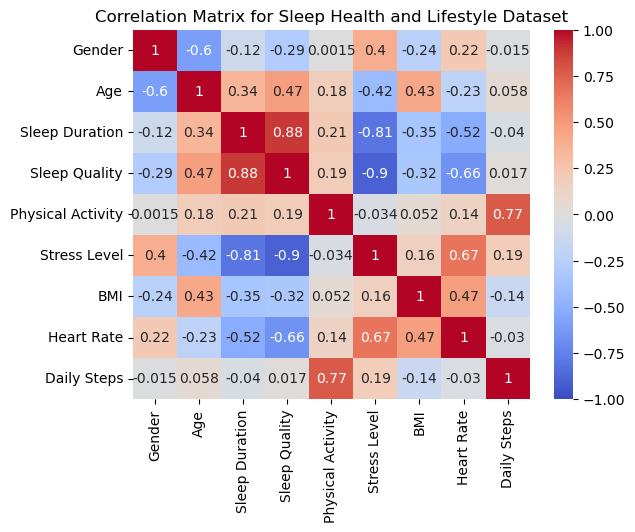
\includegraphics[width=0.60\textwidth]{correlation.png}
        \caption{Correlation Matrix}
        \label{fig:correlation}
    \end{figure}

    \noindent From these insights, it became evident that Sleep Quality and Sleep Duration were pivotal predictors of stress in our models. The potential synergistic predictive power of using these two attributes together became apparent and, for that reason, we opted to use Sleep Quality and Sleep Duration as our predictors.\\
    
    \noindent We also performed some outlier detection on these important variables using box plot models. We found no significant outliers neither in the predictor variables nor in the dependent variable Stress Level. Although Stress Level could be a value from 1 to 10, the only outcome values available from this dataset were between 3 and 8.\\
    
    \section*{Proposed Methodology}
    \noindent Given our objective to predict stress levels across six categories (levels 3-8), we are dealing with a multi-class classification problem. Upon reviewing the pair plots (\hyperref[fig:pairplot]{Figure~\ref*{fig:pairplot}}), certain graphs, such as Sleep Quality vs Sleep Duration, Sleep Duration vs Gender, and Sleep Duration vs Age indicated optimal separability in the data. We did not perform data normalization since all the values of our inputs were of equal scale and with the models chosen, normalization was not necessary. Also, no standardization was necessary because all the data we used for our models were numerical and categorical. \\

    \noindent Managing the numerous levels of our outcome variable, Stress Level, made it difficult to discern a clear distinction between our labels. To simplify the problem, we contemplated grouping levels (e.g. combining 3 and 4, 5 and 6, 7 and 8 to create three stress levels instead of six). However, we ultimately decided against grouping to avoid potential oversimplification and instead retained the original range of 3-8.\\

    \noindent After having finalized our predictors and prediction values, we plan to construct four different models using Linear Regression (LR), Multinomial Logistic Regression, a Naive Bayes Classifier (NB), and a Linear Support Vector Machine (SVM). We will then proceed to split the preprocessed data with an 80-20 train-test ratio and train them accordingly using cross-validation for LR and MLR. Cross-validation can pose computational challenges, particularly with an increasing number of folds because the process may become time-consuming, especially if the model is intricate or computational resources are constrained.\\

    \noindent Afterward, to evaluate the models, we will be using MSE and R$^2$ for LR and a classification report consisting of Precision, Recall, F1-Score, and Accuracy for the other three models. These metrics serve as indicators to evaluate the quality and performance of our models. With these values in mind, we will ultimately decide which model is the best predictive model for our dataset and compare our findings with those from previous research. Lastly, we will build a frontend to display our model predictions based on the provided user inputs.
    
    \section*{Experimental Results}

    \noindent\subsection*{Linear Regression:}

    \begin{figure}[H]
        \centering
        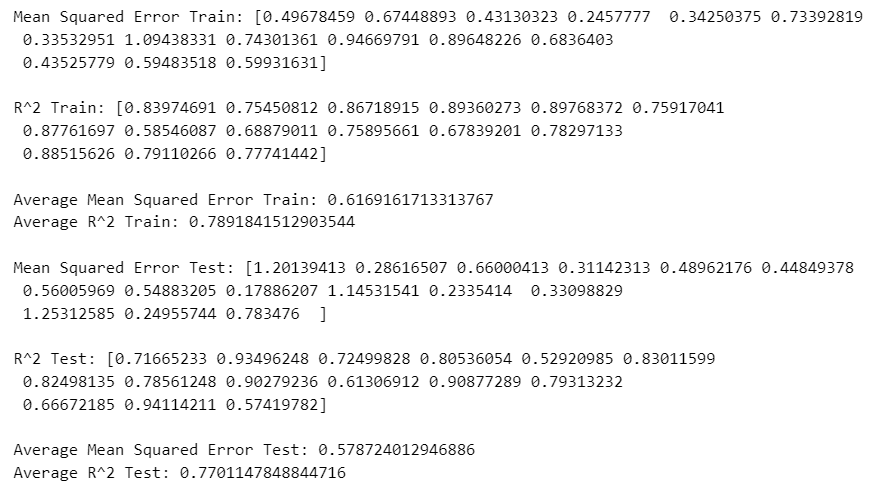
\includegraphics[width=\columnwidth]{lr-report.png}
        \caption{MSE and R$^2$ Results for Linear Regression}
        \label{fig:class-report-lr}
    \end{figure}

    \begin{figure}[H]
        \centering
        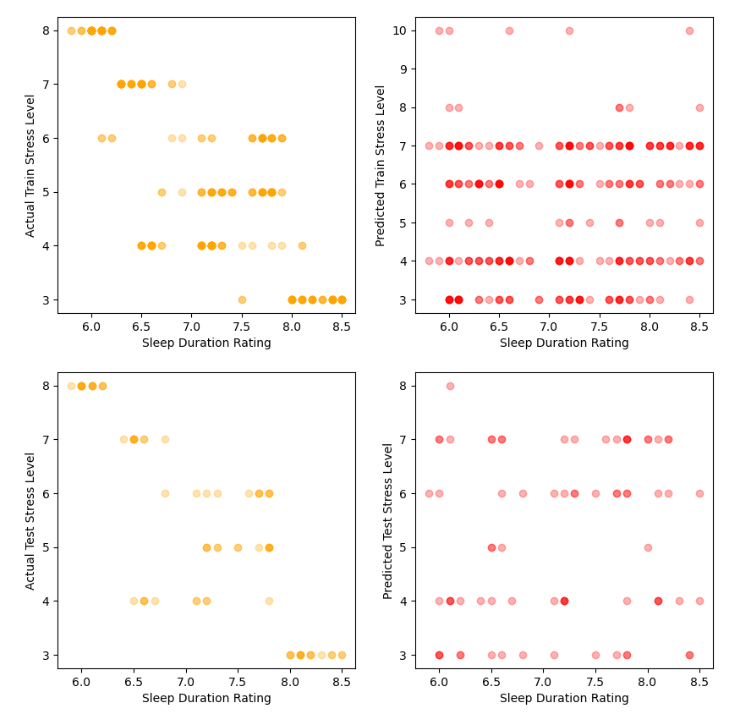
\includegraphics[width=\columnwidth]{lr-scatterplot.png}
        \caption{Scatterplot of Linear Regression}
        \label{fig:scatterplot-lr}
    \end{figure}

    \noindent The Linear Regression model underwent 15-fold cross-validation, with MSE and  R{$^2$} as performance metrics. In training, MSE averaged 0.5977, indicating a 0.598-unit deviation between predictions and actual values. R${^2}$ values ranged from 0.6207 to 0.9364, averaging 0.7909, signifying 79.1\% variance explanation. Test data MSE averaged 0.7041, slightly exceeding training data, suggesting potential overfitting. Test data R${^2}$ ranged from -6.5406 to 0.9775, averaging -0.0226, indicating limited explanatory power. 
    \noindent In summary, the model showed decent training performance but struggled to generalize, suggesting potential overfitting and necessitating further analysis and alternative approaches for improvement.
    
    \noindent\subsection*{Multinomial Logistic Regression:}
    
    \begin{figure}[H]
        \centering
        \subfloat[\centering Training Report]{{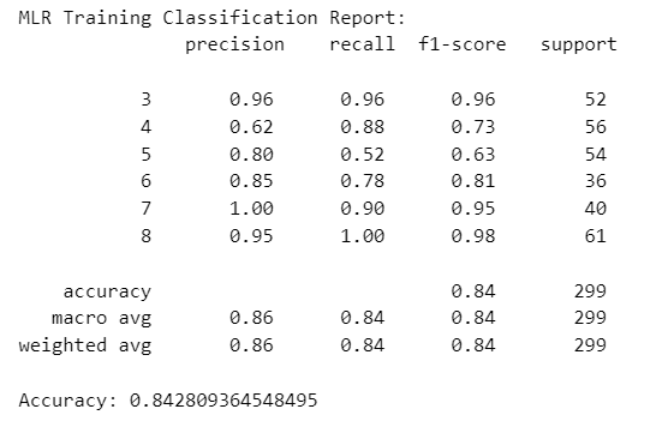
\includegraphics[width=\columnwidth]{mlr-class-report-train.png} }}
        \qquad
        \subfloat[\centering Testing Report]{{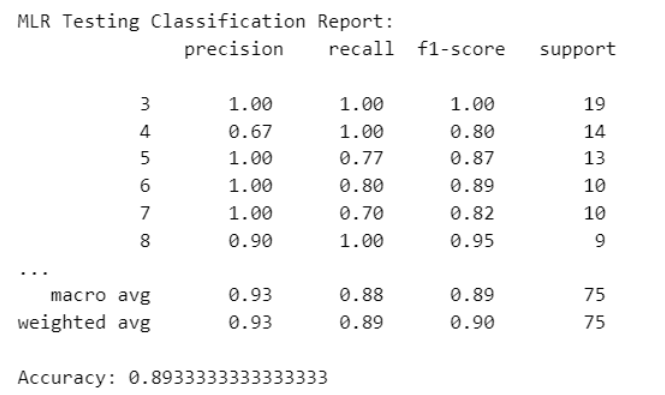
\includegraphics[width=\columnwidth]{mlr-class-report-test.png} }}
        \caption{Classification Report of Multinomial Logistic Regression}
        \label{fig:class-report-mlr}
    \end{figure}

    \begin{figure}[H]
        \centering
        \subfloat[\centering Confusion Matrix for Training Data]{{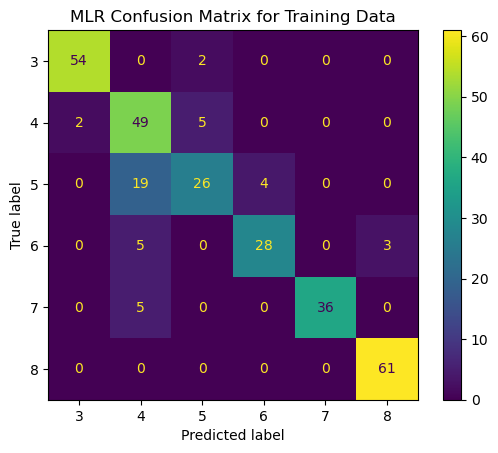
\includegraphics[width=\columnwidth]{mlr-confusion-matrix-train.png} }}
        \qquad
        \subfloat[\centering Confusion Matrix for Testing Data]{{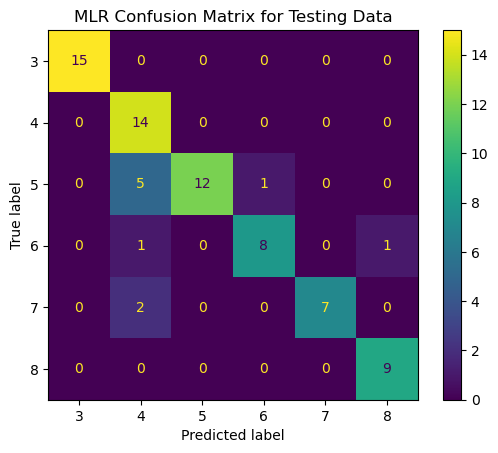
\includegraphics[width=\columnwidth]{mlr-confusion-matrix-test.png} }}
        \caption{Confusion Matrix of Multinomial Logistic Regression}
        \label{fig:confusion-matrix-mlr}
    \end{figure}

    \noindent The Logistic Regression model, built using sklearn’s LogisticRegressionCV function, demonstrated strong performance across most classes in training and test sets. From the classification report, classes 3, 7, and 8 have high precision, recall, and f1-score in both sets indicating the precise classification of these classes. However, class 4 showed a lower precision than the other classes in both sets, but a higher recall indicates a higher likelihood of false positives.\\
    
    \noindent The overall accuracy of the training set is approximately 84.28\%, while the test set accuracy is 89.33\%. However, the lower precision of class 4 impacts the overall accuracy of both sets, so there is room for improvement. These high accuracy scores demonstrate the model’s ability to correctly classify class labels for a significant portion of the instances in both seen and unseen data. 
    
    \noindent\subsection*{Naive Bayes:}

    \begin{figure}[H]
        \centering
        \subfloat[\centering Training Report]{{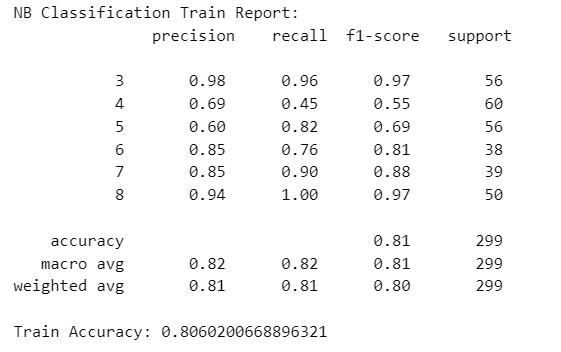
\includegraphics[width=7.5cm]{nb-class-report-train.png} }}
        \qquad
        \subfloat[\centering Testing Report]{{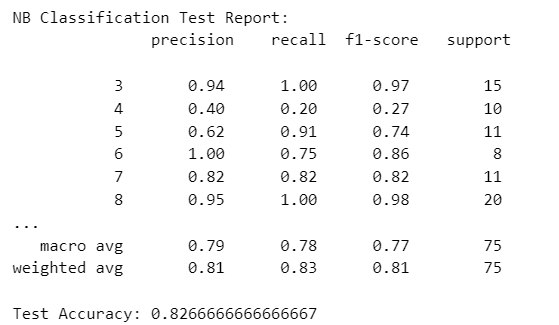
\includegraphics[width=7.5cm]{nb-class-report-test.png} }}
        \caption{Classification Report of Naive Bayes}
        \label{fig:class-report-nb}
    \end{figure}

    \begin{figure}[H]
        \centering
        \subfloat[\centering Confusion Matrix for Training Data]{{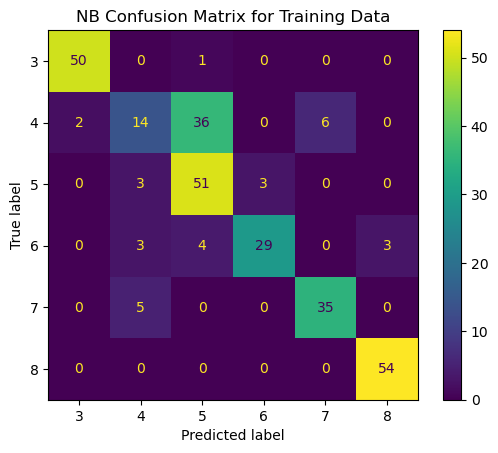
\includegraphics[width=\columnwidth]{nb-confusion-matrix-train.png} }}
        \qquad
        \subfloat[\centering Confusion Matrix for Testing Data]{{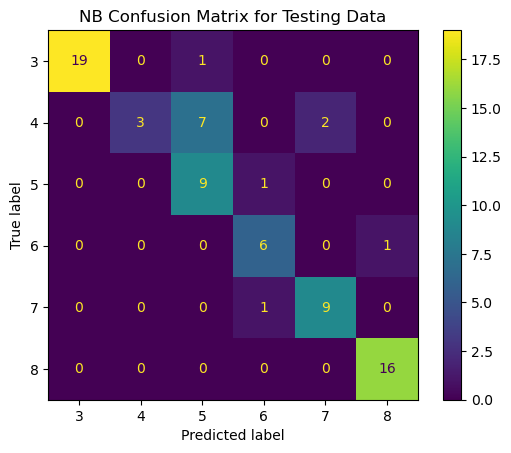
\includegraphics[width=\columnwidth]{nb-confusion-matrix-test.png} }}
        \caption{Confusion Matrix of Naive Bayes}
        \label{fig:confusion-matrix-nb}
    \end{figure}

    \noindent The Naive Bayes model, built using sklearn’s GaussianNB function demonstrated mixed performance across classes in training and test datasets. From the classification report, classes 3 and 8 have high precision, recall, and f1-score that is all above 0.9 in both sets. This indicates strong and precise classification of these classes. However, classes 4 and 5 showed a lower precision, with class 4 also having low recall, indicating inaccurate classification for these classes.\\
    
    \noindent The overall accuracy of the training set is approximately 80.60\%, while the test set accuracy is 82.67\%. This suggests a relatively better performance when classifying unseen data. There is room for enhancing the model’s performance, particularly in accurately classifying instances for classes 4 and 5.
    
    \noindent\subsection*{Linear Support Vector Machine:}

    \begin{figure}[H]
        \centering
        \subfloat[\centering Training Report]{{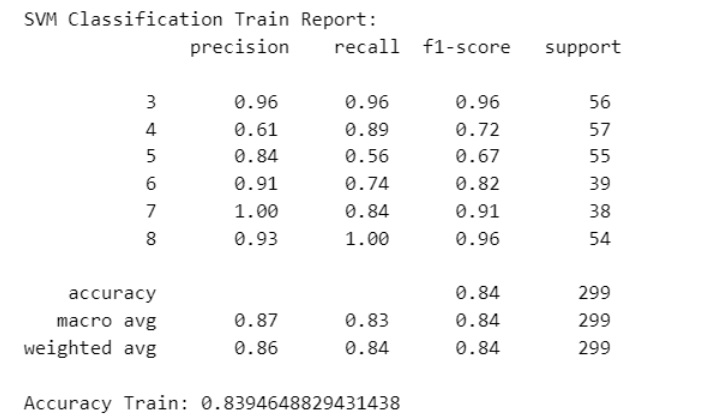
\includegraphics[width=\columnwidth]{svm-class-report-train.png} }}
        \qquad
        \subfloat[\centering Testing Report]{{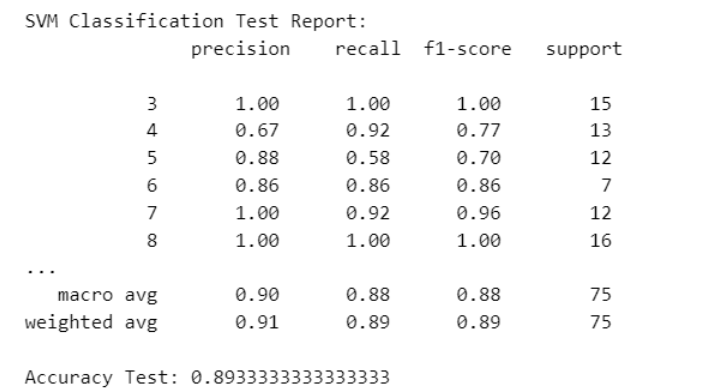
\includegraphics[width=\columnwidth]{svm-class-report-test.png} }}
        \caption{Classification Report of Linear Support Vector Machine}
        \label{fig:class-report-svm}
    \end{figure}

    \begin{figure}[H]
        \centering
        \subfloat[\centering Confusion Matrix for Training Data]{{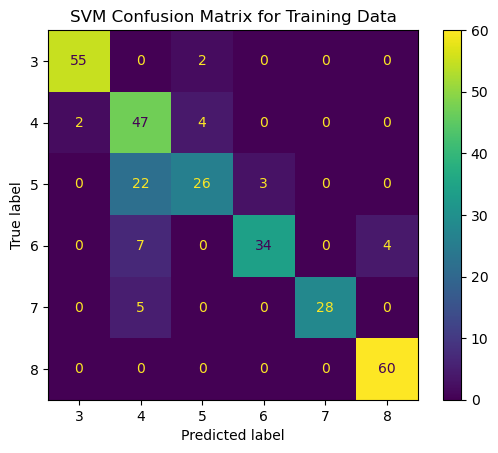
\includegraphics[width=\columnwidth]{svm-confusion-matrix-train.png} }}
        \qquad
        \subfloat[\centering Confusion Matrix for Testing Data]{{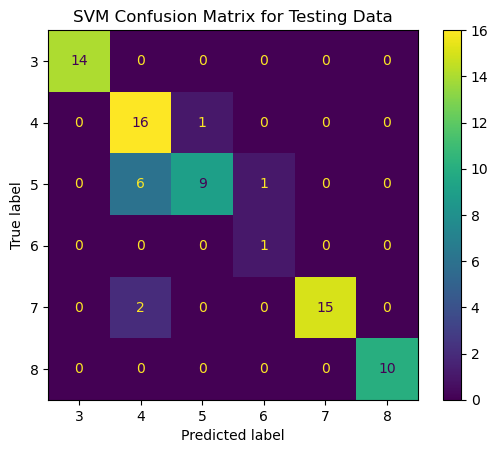
\includegraphics[width=\columnwidth]{svm-confusion-matrix-test.png} }}
        \caption{Confusion Matrix of Linear Support Vector Machine}
        \label{fig:confusion-matrix-svm}
    \end{figure}


    \noindent We utilized sklearn's SVC function to implement the Support Vector Machine (SVM) for our analysis. The SVM model employs a Radial Basis Function (RBF) kernel.\\

    \noindent In the training set, the model demonstrated a high precision of 0.97 for class 3, with commendable recall and F1-score, also at 0.97. Conversely, class 4 exhibited a lower precision of 0.64, coupled with a high recall of 0.91. The overall training set accuracy was 83.95\%. In the test set, the model maintained strong precision, achieving a perfect 1.00 for classes 3 and 8. However, class 4 had lower precision at 0.67, with a high recall of 0.92, echoing the training set trend. The overall test set accuracy was 89.33\%.\\
    
    \noindent In summary, the SVM model displayed commendable performance in classifying the dataset, with elevated precision, recall, and F1-scores across most classes. There is still room for improvement in the model's performance for class 4. Despite that, the model's consistent accuracy on both the training and test sets suggests its effectiveness and ability to generalize well to unseen data.

    \noindent\subsection*{Software Implementation:}
    
    \noindent For software implementation, we utilized Next.js and Flask to construct our web page for testing and running our model. The component receives two inputs, namely sleep quality and sleep duration. It subsequently initiates a POST request to the '/api/predict' API endpoint with these inputs. The API then employs four distinct machine learning models (i.e. Linear Regression, Multinomial Logistic Regression, Naive Bayes, and Linear Support Vector Machine) to make predictions. These models, having been pre-trained, are loaded from a pickle file. Following the prediction process, the results are returned to the front end as a JSON response and displayed.

    \begin{figure}[H]
        \centering
        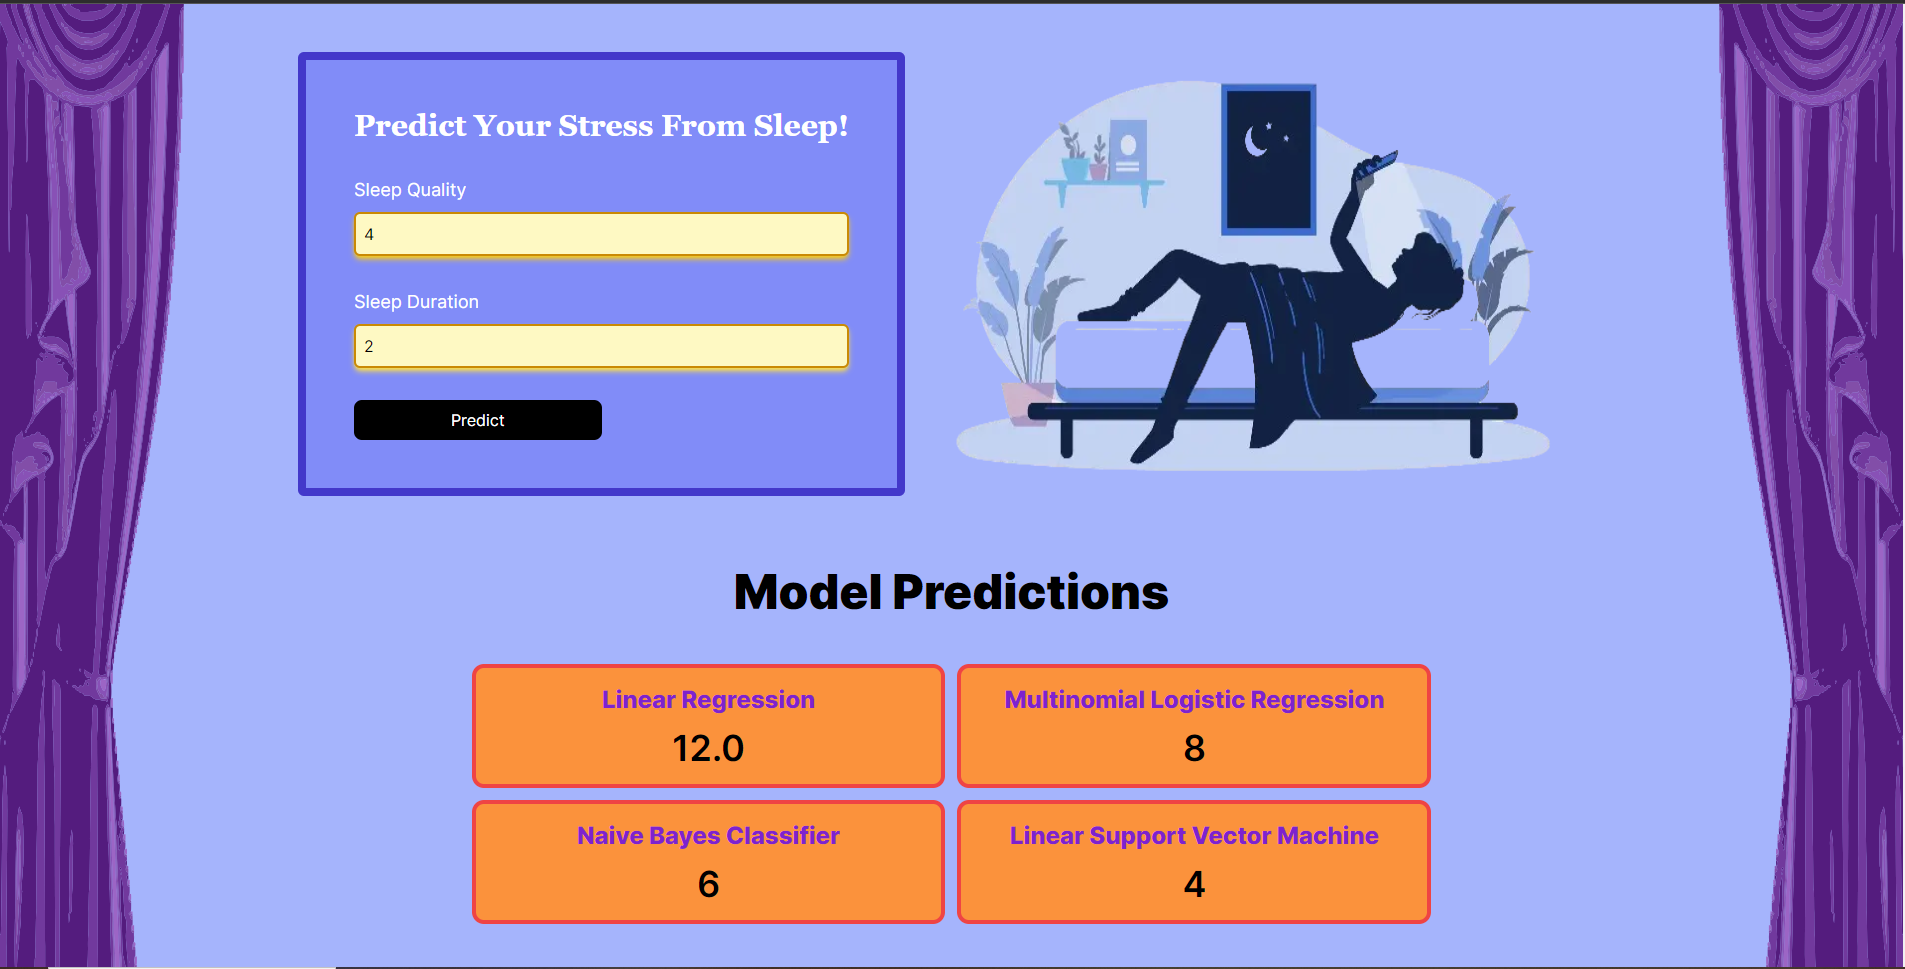
\includegraphics[width=\columnwidth]{frontend.png}
        \caption{Demo of Frontend}
        \label{fig:frontend}
    \end{figure}

    \section*{Conclusion and Discussion}
    \noindent Using the “Sleep Health and Lifestyle Dataset” and four models (Linear Regression, Logistic Regression, Naive Bayes, and Support Vector Machine), we formed models predicting Stress Level. While Linear Regression fell short, Multinomial Logistic Regression, Naive Bayes, and SVM achieved over 80\% accuracy, particularly excelling at predicting levels 3, 6, 7, and 8. Notably, Multinomial Logistic Regression and SVM emerged as the best predictive models, aligning with prior research. It seems that Logistic Regression had a slightly better performance than NonLinear SVM. This could be due to the fact that Logistic Regression uses thresholds on the data in order to make a prediction unlike SVM, which extrapolates the data into another higher dimension to make predictions. This extrapolation could result in introducing error into the model, explaining why SVM performs a bit poorer than Logistic Regression. In stark contrast, however, we found that Naive Bayes was the worst out of the three contenders in comparison to external studies that concluded with Naive Bayes having the best predictive capabilities amongst all of their models. This can be attributed to many factors (e.g. our way of categorization, training and testing, etc).\\
    
    \noindent For the future of stress prediction with machine learning, it is recommended that more robust models, along with a larger training set (possibly from real data), are used for practicality and to get less ambiguous trends. Furthermore, creating and testing other types of models, such as Decision Trees or Multilayer Perceptrons (MLPs), may yield slightly more accurate predictions than the models developed in this project. Regardless of what the future might bring, we take pride in what we’ve accomplished over the span of 10 weeks, transitioning from a collection of ideas to creating predictive models with accuracies exceeding 80\%, and ultimately developing a fully functioning frontend to display their capabilities.

    \begin{thebibliography}{9}
        \bibitem{bib:1} M. M. Rahman, A. Mohaimenul Islam, J. Miah, S. Ahmad, and M. Mamun, “Sleepwell:stress level prediction through sleep data. are you stressed?,” 2023 IEEE World AI IoT Congress (AIIoT), 2023. doi:10.1109/aiiot58121.2023.10174306.\\

        \bibitem{bib:2} S. Jayawickrama and S. Rupasingha, “Predicting stress levels using sleep data,” 2019 IEEE 19th International Conference on Bioinformatics and Bioengineering (BIBE), 2019. doi:10.1109/bibe.2019.000-9.\\

        \bibitem{bib:3} L. Tharmalingam, “Sleep Health and Lifestyle Dataset,” Kaggle, 2021. [Online]. Available: https://www.kaggle.com/lahiripremarathne/sleep-health-and-lifestyle-dataset. [Accessed: 10-Jun-2021].\\

    \end{thebibliography}

    \begin{table*}[hbt!]
        \centering
            \begin{tabular}{l|c|c|c}
                \hline \hline
                \multicolumn{4}{c}{\textbf{Project Roadmap}} \\ % resizes n columns into one
                \hline \hline
                \multicolumn{1}{c|}{\textbf{Task}} & \textbf{Start Date} & \textbf{End Date} & \textbf{Duration (days)} \\
                \hline
                Background/Literature Review & Oct. 16 & Oct. 22 & 7 \\
                \hline
                Exploratory Data Analysis & Oct. 23 & Oct. 29 & 7 \\
                \hline
                Developing prediction models & Oct. 30 & Nov. 8 & 10 \\
                \hline
                Evaluation of the model and testing performance & Nov. 9 & Nov. 14 & 9 \\
                \hline
                Developing front-end to display and run models & Nov. 15 & Nov. 27 & 12 \\
                \hline
                Writing Report & Nov. 9 & Dec. 6 & 34 \\
                \hline
                Presentation Practice & Dec. 2 & Dec. 5 & 3 \\
                \hline \hline
            \end{tabular}
            \caption{Tasks, Start and End Dates, and Duration}
        \label{tab:timeline}
    \end{table*}

\end{document}